\chapter{Plataforma Codeboard UERJ}
% Revisado

A plataforma Codeboard UERJ é uma ferramenta de ensino de programação que permite a criação de salas de aula virtuais, onde os alunos podem escrever códigos de programação em tempo real. A plataforma foi desenvolvida com base em três princípios fundamentais: colaboração, interatividade e praticidade. Ela foi projetada para ser simples e intuitiva, permitindo que os usuários a utilizem sem a necessidade de treinamento prévio. 

Este capítulo apresenta a plataforma Codeboard UERJ e nele serão abordados os objetivos, funcionalidades e a arquitetura da plataforma.	

\section{Objetivos}
% Revisado

O objetivo principal da plataforma Codeboard UERJ é auxiliar no ensino de programação, permitindo que professores criem e gerenciem atividades práticas para seus alunos. A plataforma foi desenvolvida para ser utilizada em disciplinas de programação de computadores, como Algoritmos e Estruturas de Dados, Linguagens de Programação e Paradigmas de Programação.

A motivação para o desenvolvimento da plataforma surgiu durante a pandemia de COVID-19, quando as aulas presenciais foram suspensas e as atividades práticas de programação tiveram que ser adaptadas para o ensino remoto. Ela foi desenvolvida para atender a essa demanda, dando a capacidade aos professores de acompanharem o progresso dos alunos e avaliarem suas atividades práticas em tempo real.


\section{Funcionalidades}
% Revisado

Para atingir os objetivos propostos, o desenvolvimento da plataforma foi restrito a um conjunto de funcionalidades essenciais, que são:
Autenticação de usuários, gerenciamento de salas e seus participantes e o quadro de programação em tempo real.

\subsection{Autenticação de Usuários}
% Revisado

O sistema de autenticação de usuários é o ponto de partida para o uso da plataforma, permitindo que novos usuários se cadastrem e realizem login para acessar suas funcionalidades. O processo de cadastro ocorre por meio de um formulário que coleta informações básicas, como nome, e-mail e senha. Após a conclusão do cadastro, o usuário está apto a realizar login utilizando o e-mail e a senha fornecidos.

Durante o login, a plataforma valida as credenciais inseridas, verificando se o e-mail e a senha correspondem a uma conta existente. Se os dados forem corretos, o usuário é autenticado e direcionado à página inicial. Caso contrário, uma mensagem de erro é exibida, informando que as credenciais são inválidas. Caso o usuário ainda não tenha uma conta, ele pode acessar a página de cadastro por meio de um link, preencher o formulário e, após o registro, ser redirecionado automaticamente para a tela inicial. Esse processo de autenticação está ilustrado no diagrama de fluxo da Figura \ref{fig:user-auth-flow}, com as telas de login e cadastro exibidas nas Figuras \ref{fig:login-page} e \ref{fig:signup-page}, respectivamente.

\begin{figure}[H]{0.8\textwidth}
    \centering
    \caption{Diagrama do fluxo de autenticação de usuários.}
    \label{fig:user-auth-flow}
    \includegraphics[width=1\textwidth]{diagrams/user-auth-flow.png}
\end{figure}

\begin{figure}[H]{0.8\textwidth}
    \centering
    \caption{Página de login da plataforma Codeboard UERJ.}
    \label{fig:login-page}
    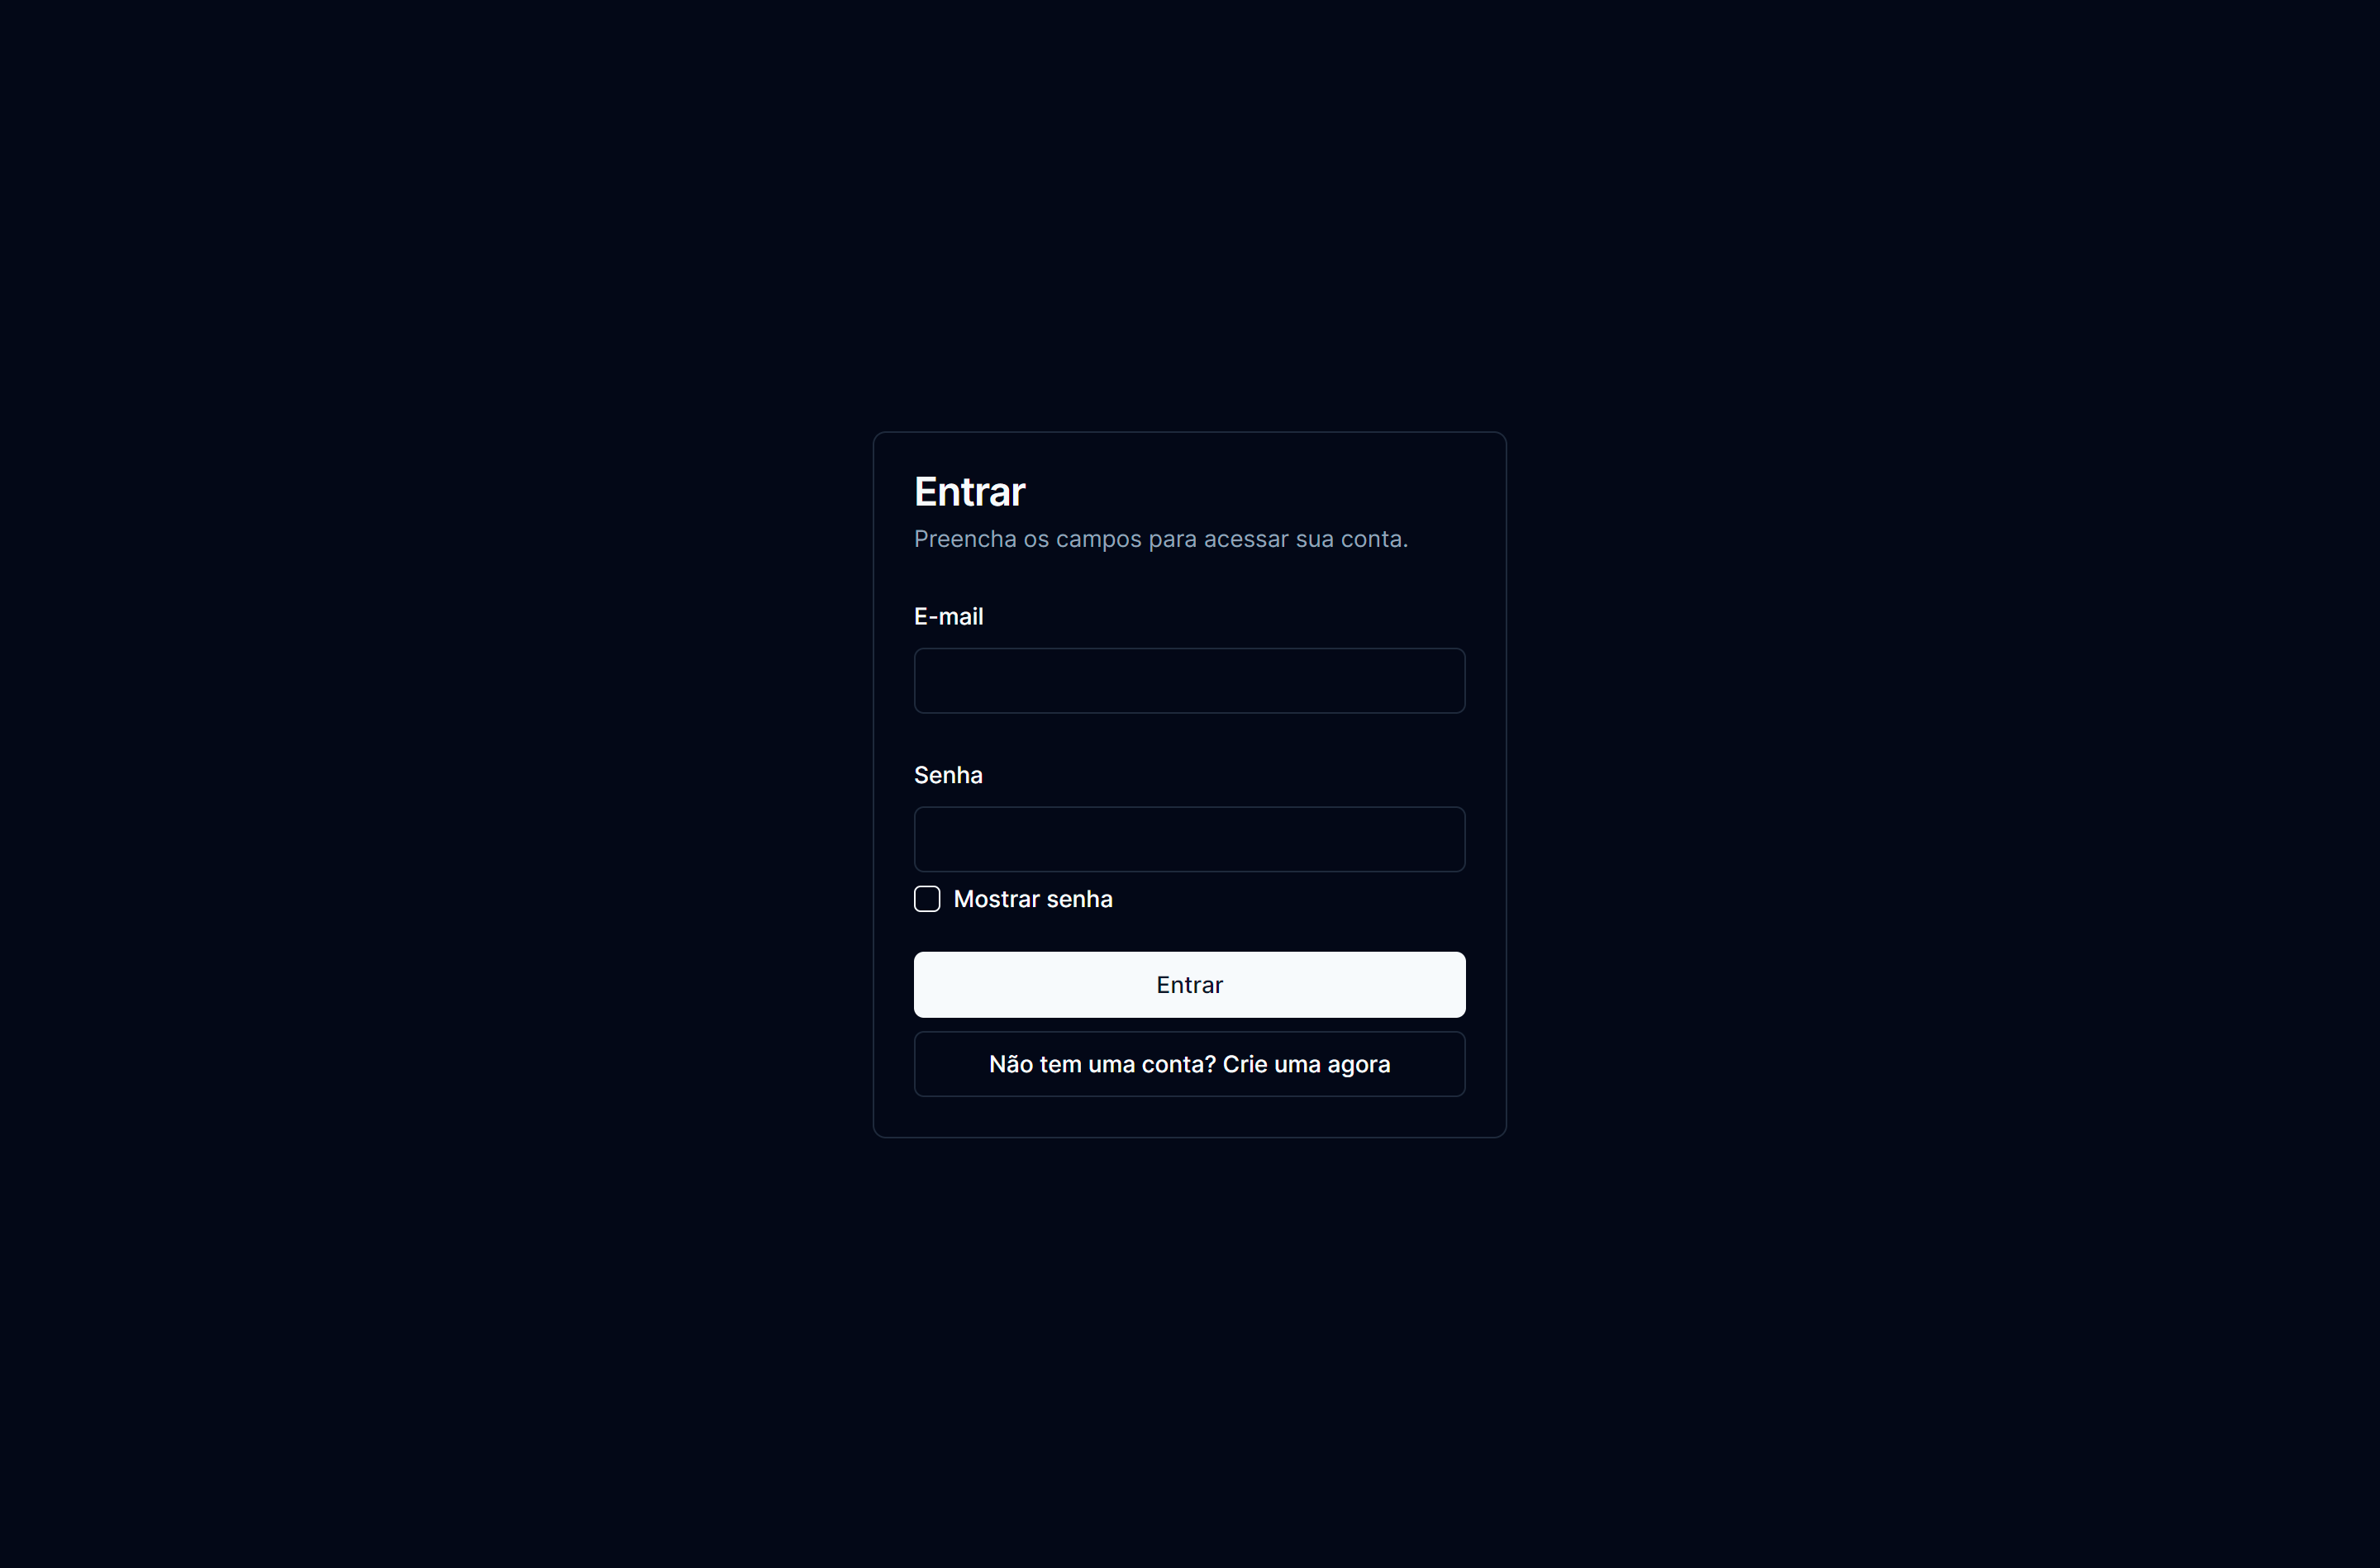
\includegraphics[width=0.8\textwidth]{assets/codeboard/login-page.png}
\end{figure}

\begin{figure}[H]{0.8\textwidth}
    \centering
    \caption{Página de cadastro da plataforma Codeboard UERJ.}
    \label{fig:signup-page}
    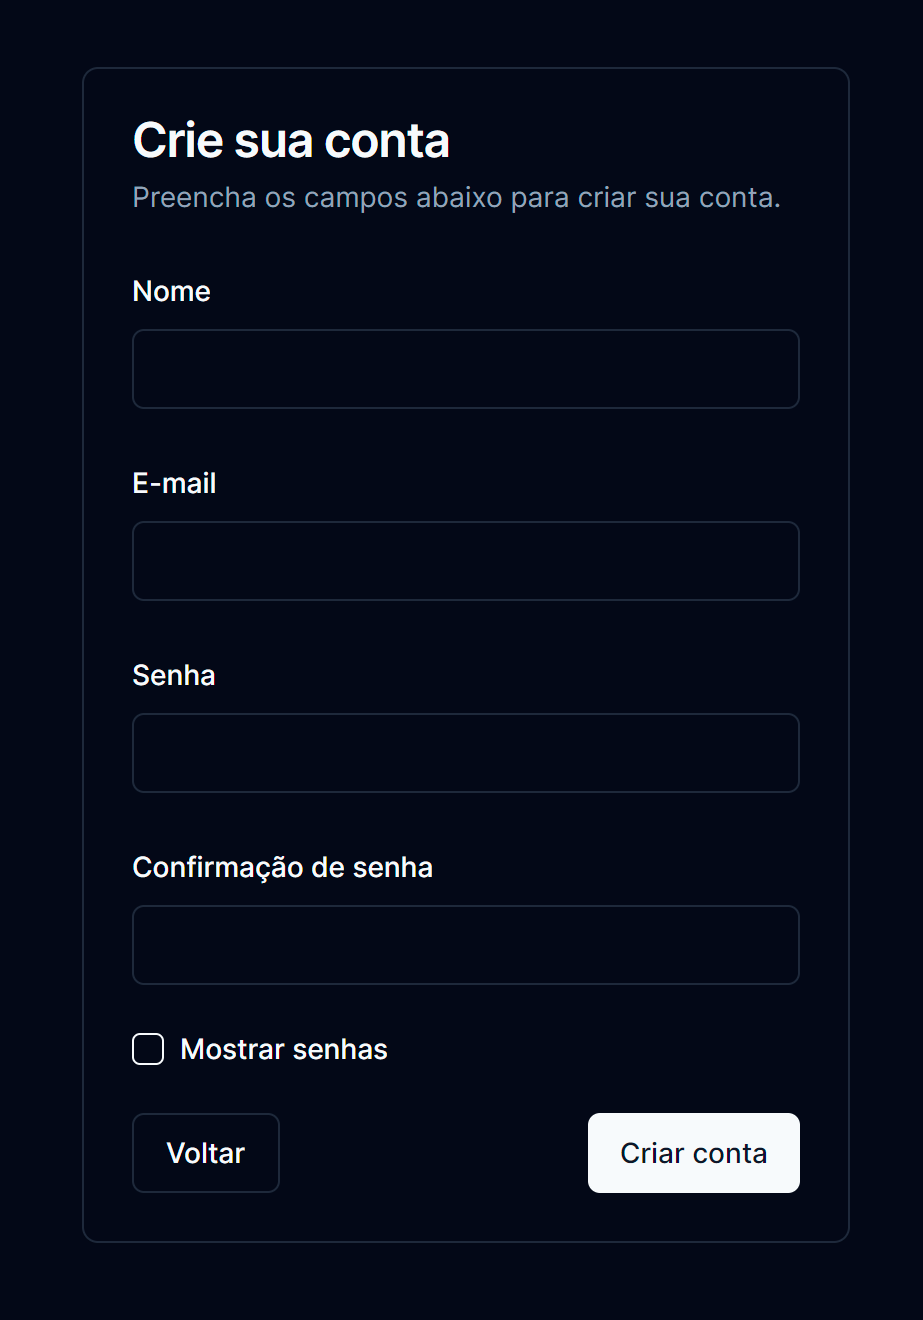
\includegraphics[width=0.8\textwidth]{assets/codeboard/signup-page.png}
\end{figure}

Durante o processo de autenticação, a plataforma utiliza tokens para manter a sessão do usuário ativa. O token é gerado no servidor e enviado ao cliente, sendo armazenado no navegador por meio de cookies. Esse token é então utilizado em todas as requisições subsequentes feitas ao servidor, garantindo que o usuário permaneça autenticado enquanto navega pelas diversas páginas da plataforma.

\subsection{Gerenciamento de Salas}
% Revisado

A funcionalidade de gerenciamento de salas, ilustrada na Figura \ref{fig:rooms-page}, constitui a página inicial da plataforma. Nessa página, as salas são apresentadas em uma lista, onde cada sala é representada por um cartão que exibe o nome, a descrição e o número de participantes. O usuário pode acessar uma sala ao clicar no respectivo cartão, sendo então redirecionado para a tela da sala.

\begin{figure}[H]{1\textwidth}
    \centering
    \caption{Página de listagem de salas da plataforma Codeboard UERJ.}
    \label{fig:rooms-page}
    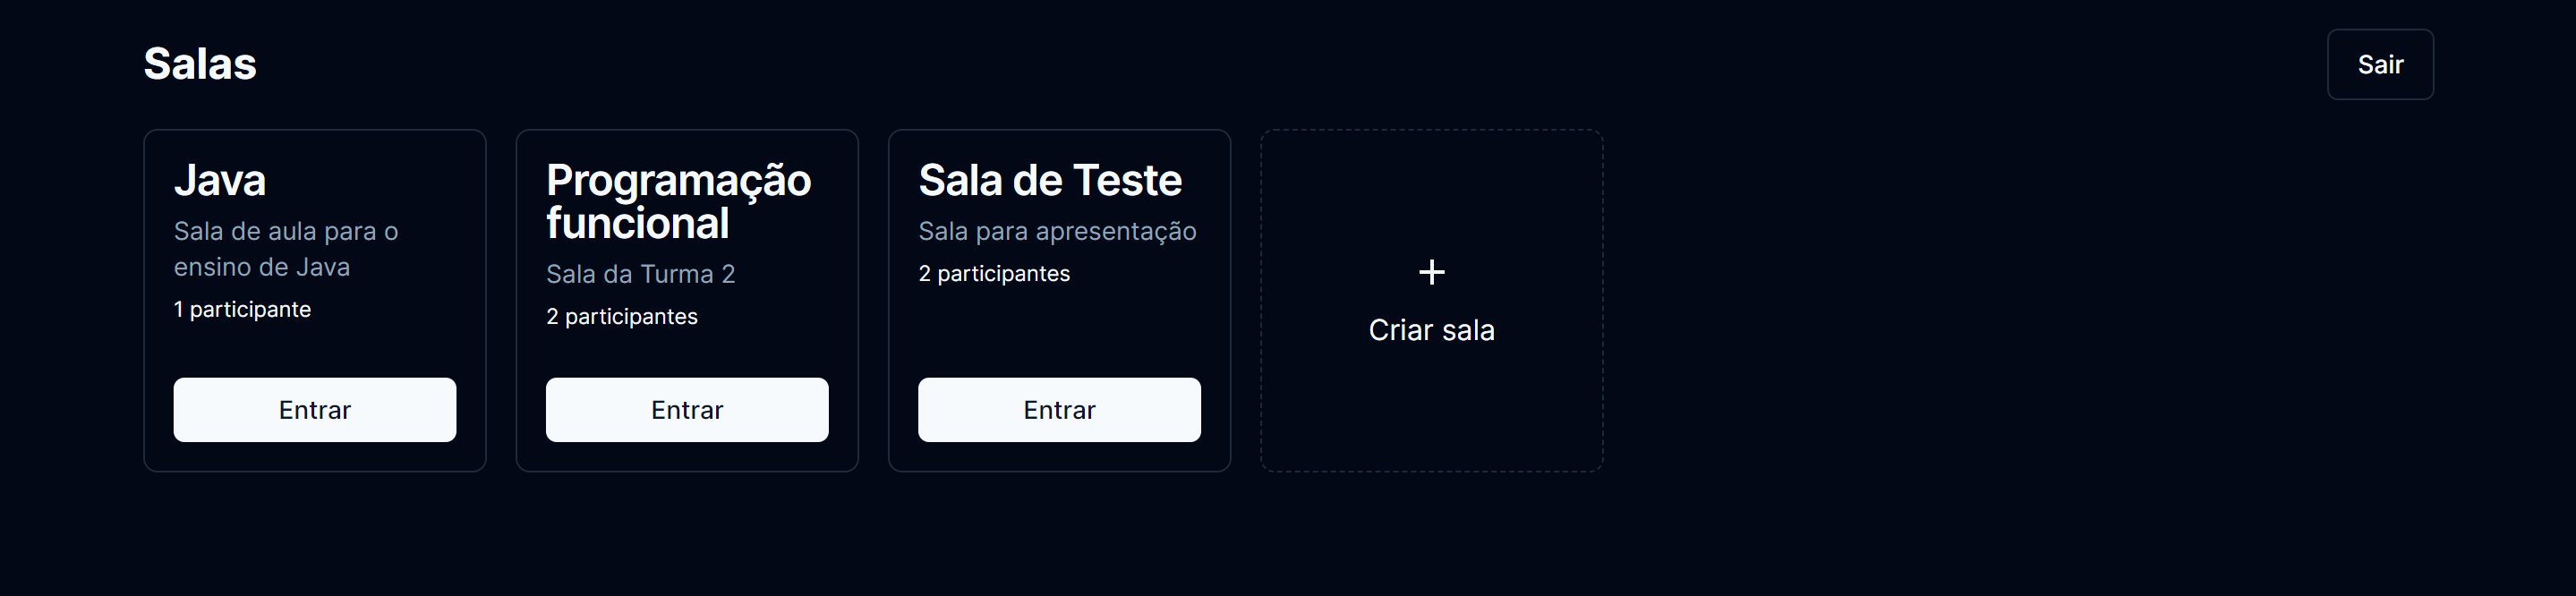
\includegraphics[width=1\textwidth]{assets/codeboard/rooms-page.png}
\end{figure}


Além disso, o usuário pode criar uma nova sala diretamente na tela inicial, utilizando o botão de criação de sala. Ao clicar no botão, o usuário é redirecionado para a página de criação de sala, mostrada na Figura \ref{fig:create-room-page}. Nessa página, é possível inserir o nome e a descrição da sala para concluir a criação.

\begin{figure}[H]{0.75\textwidth}
    \centering
    \caption{Página de criação de sala da plataforma Codeboard UERJ.}
    \label{fig:create-room-page}
    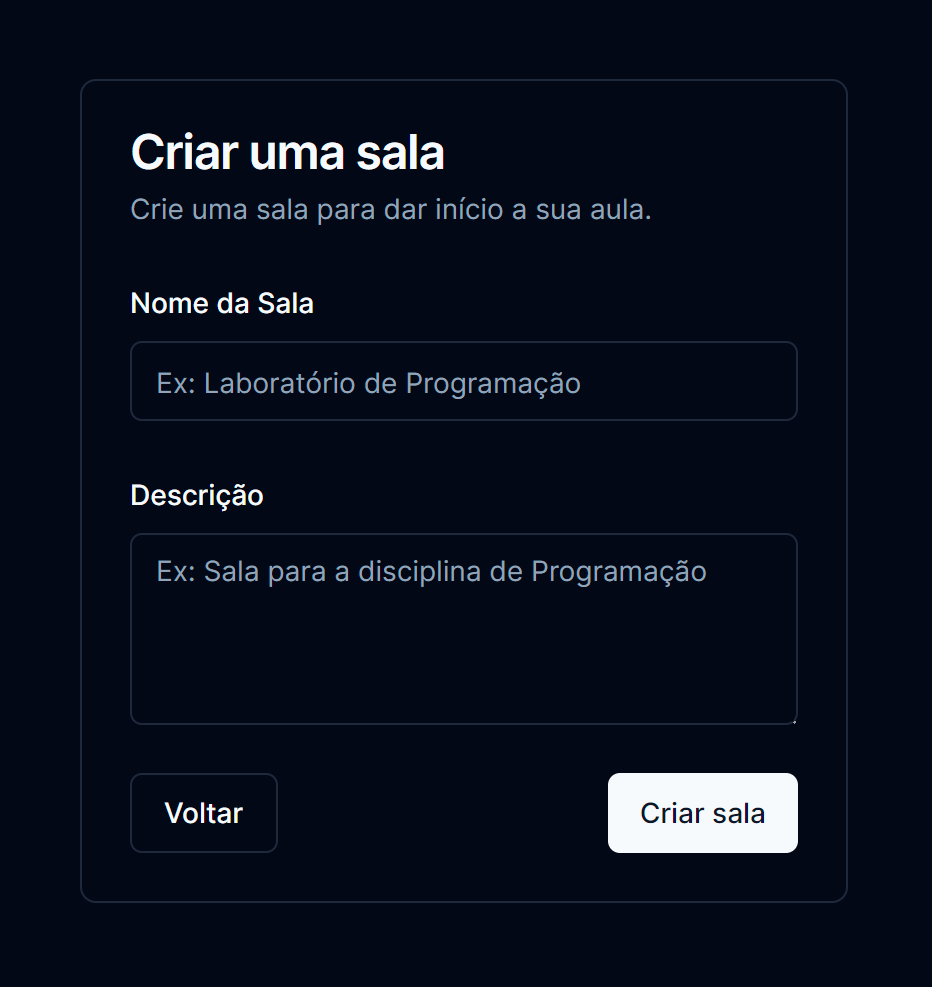
\includegraphics[width=0.75\textwidth]{assets/codeboard/create-room-page.png}
\end{figure}

Após a criação, o usuário é redirecionado para a tela da sala. Para adicionar novos membros, basta clicar no botão de adição de participantes, identificado por um ícone de usuário, conforme mostrado na Figura \ref{fig:add-member-modal}. Uma nova tela será exibida com um campo para inserção do e-mail do aluno que se deseja adicionar à sala. Após a inclusão, o aluno torna-se membro da sala e pode acessá-la.

\begin{figure}[H]{0.8\textwidth}
    \centering
    \caption{Tela de adição de alunos à sala da plataforma Codeboard UERJ.}
    \label{fig:add-member-modal}
    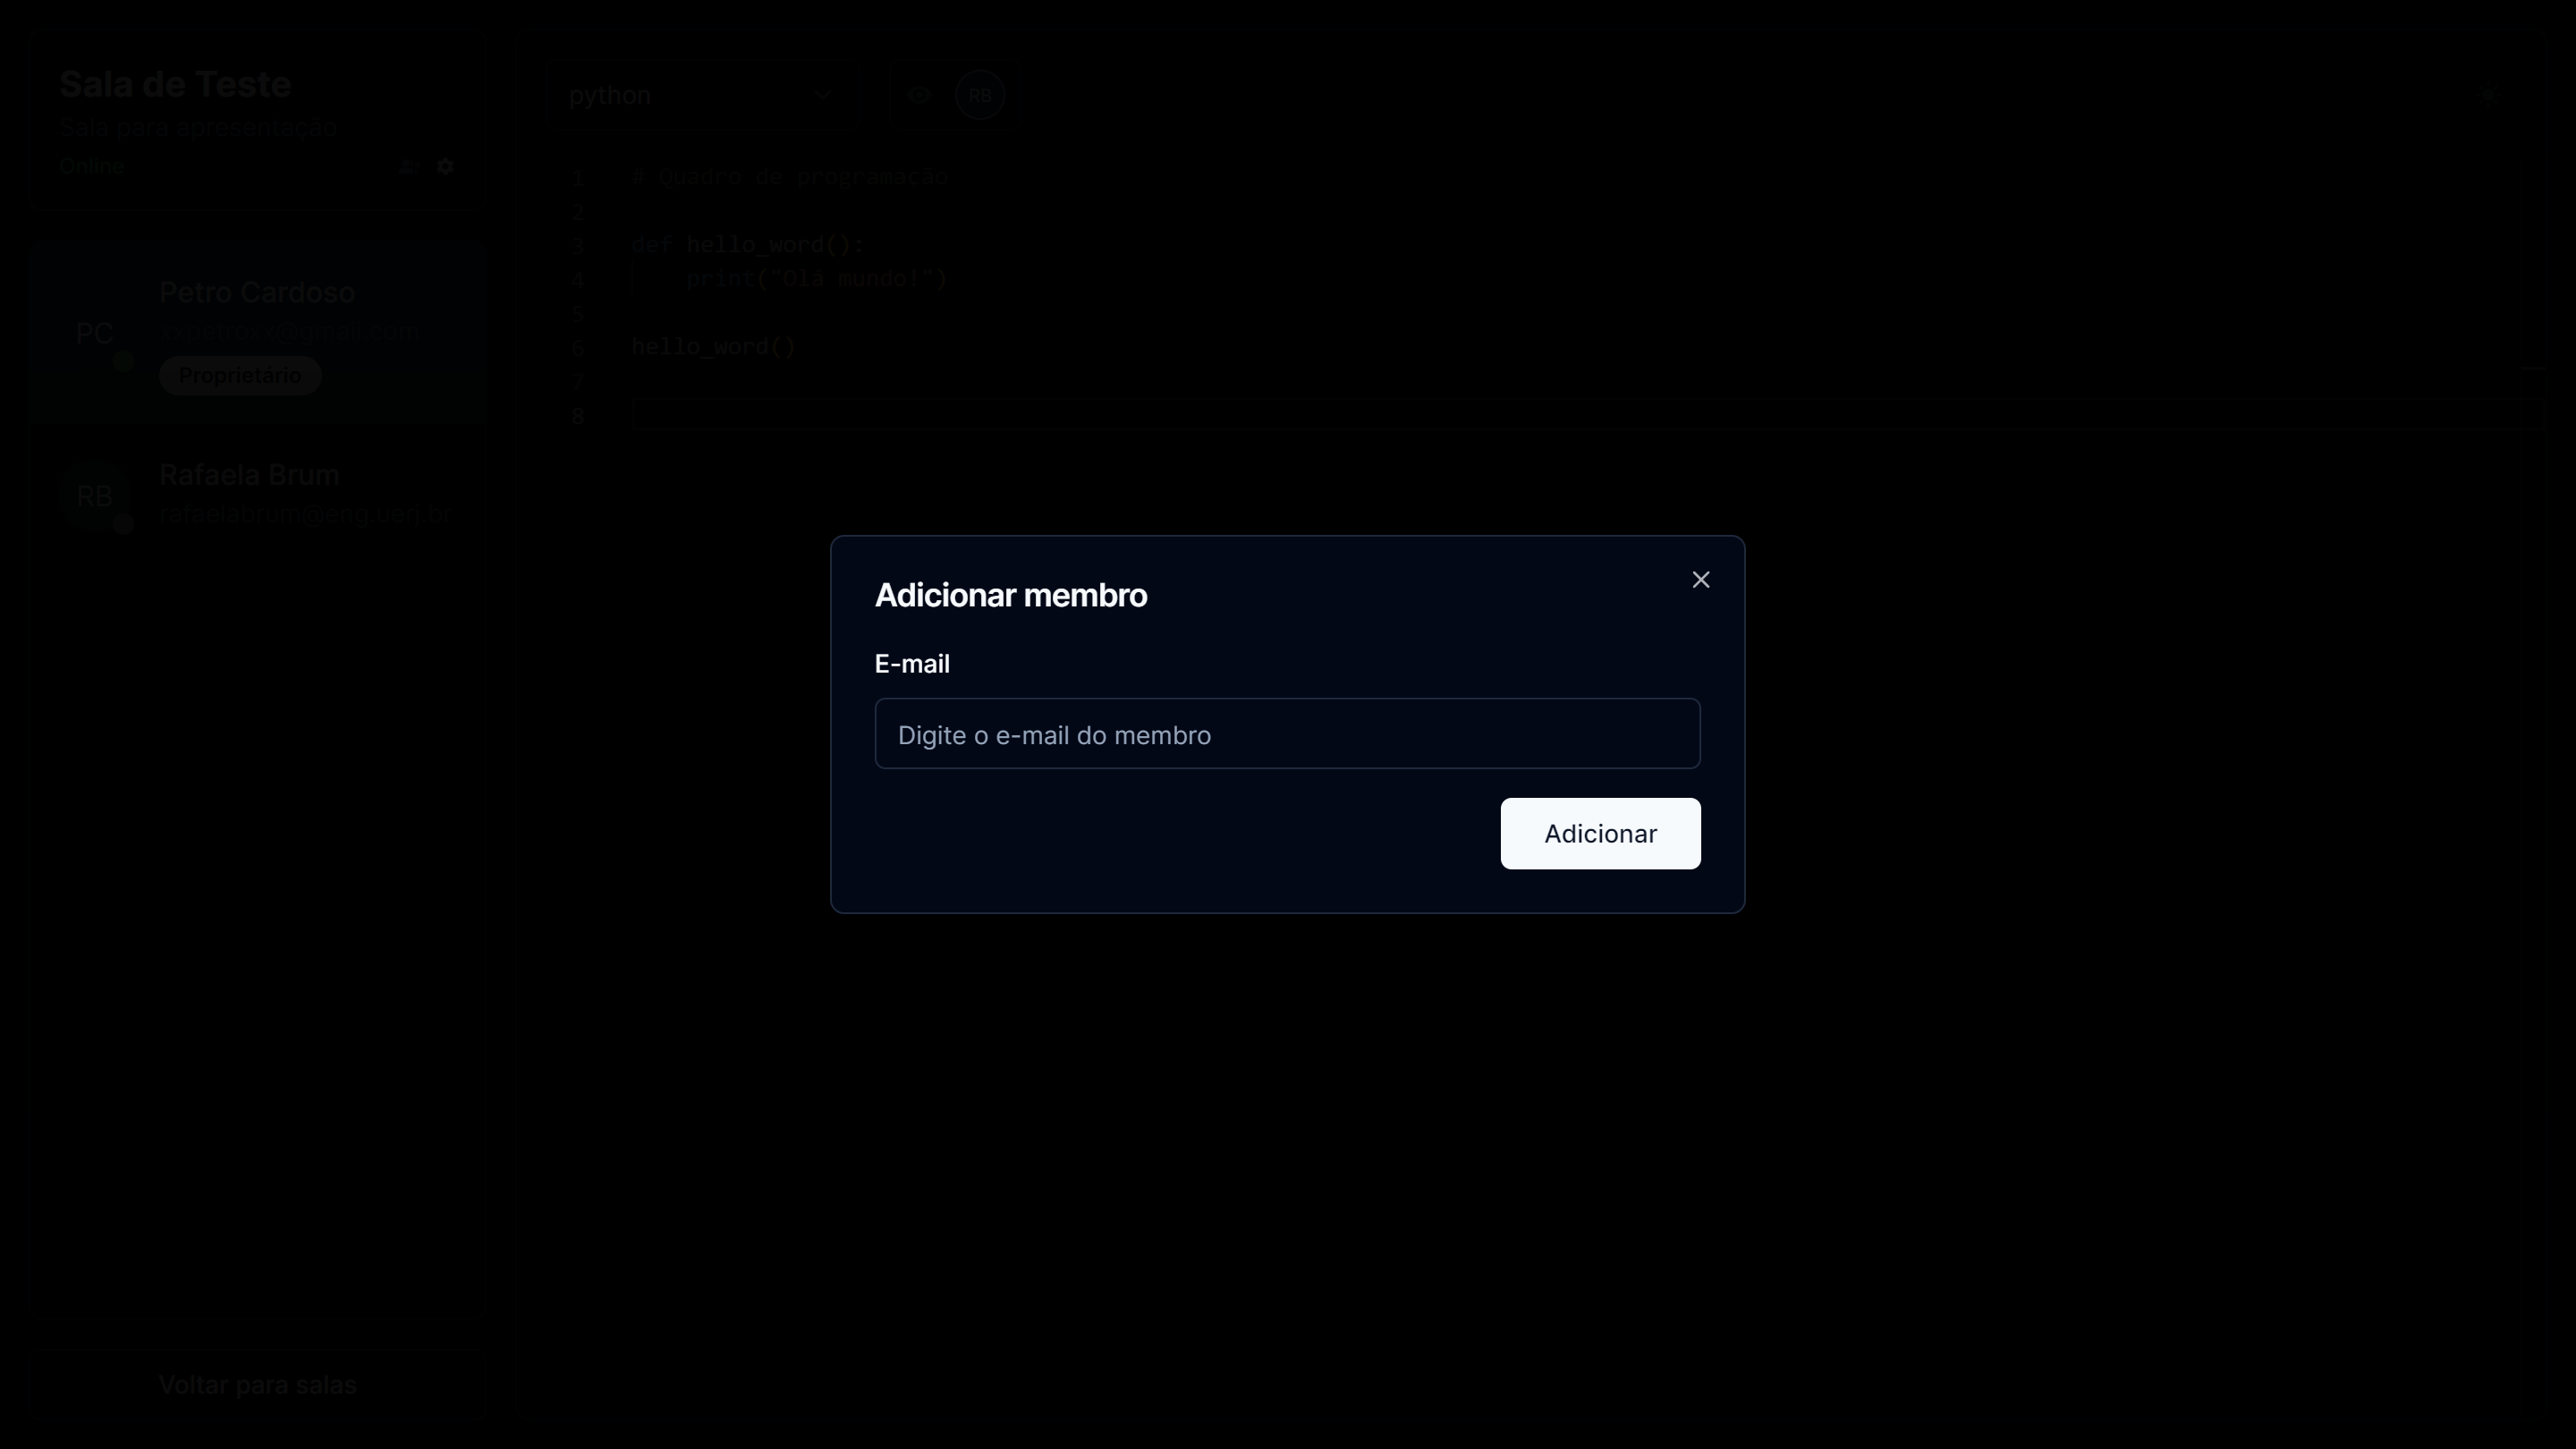
\includegraphics[width=0.8\textwidth]{assets/codeboard/add-member-modal.png}
\end{figure}


O fluxo descrito do gerenciamento de salas está representado no diagrama da Figura \ref{fig:user-room-flow}.


\begin{figure}[H]{0.85\textwidth}
    \centering
    \caption{Diagrama do fluxo de gerenciamento de salas.}
    \label{fig:user-room-flow}
    \includegraphics[width=0.85\textwidth]{diagrams/user-room-flow.png}
\end{figure}

\subsection{Quadro de Programação em Tempo Real}
% Revisado

A principal funcionalidade da plataforma é o quadro de programação em tempo real, que permite aos alunos escreverem códigos diretamente no navegador, sem a necessidade de instalar um ambiente de desenvolvimento integrado (IDE).

Para acessar o quadro de programação, o usuário deve entrar na sala desejada por meio da página de gerenciamento de salas. A plataforma exibe uma tela dividida em dois módulos: o módulo lateral, que contém a seleção de usuários, e o módulo central, onde ocorre a edição de código.

\begin{figure}[H]{1\textwidth}
    \centering
    \caption{Página da sala de programação da plataforma Codeboard UERJ.}
    \label{fig:room-details-page}
    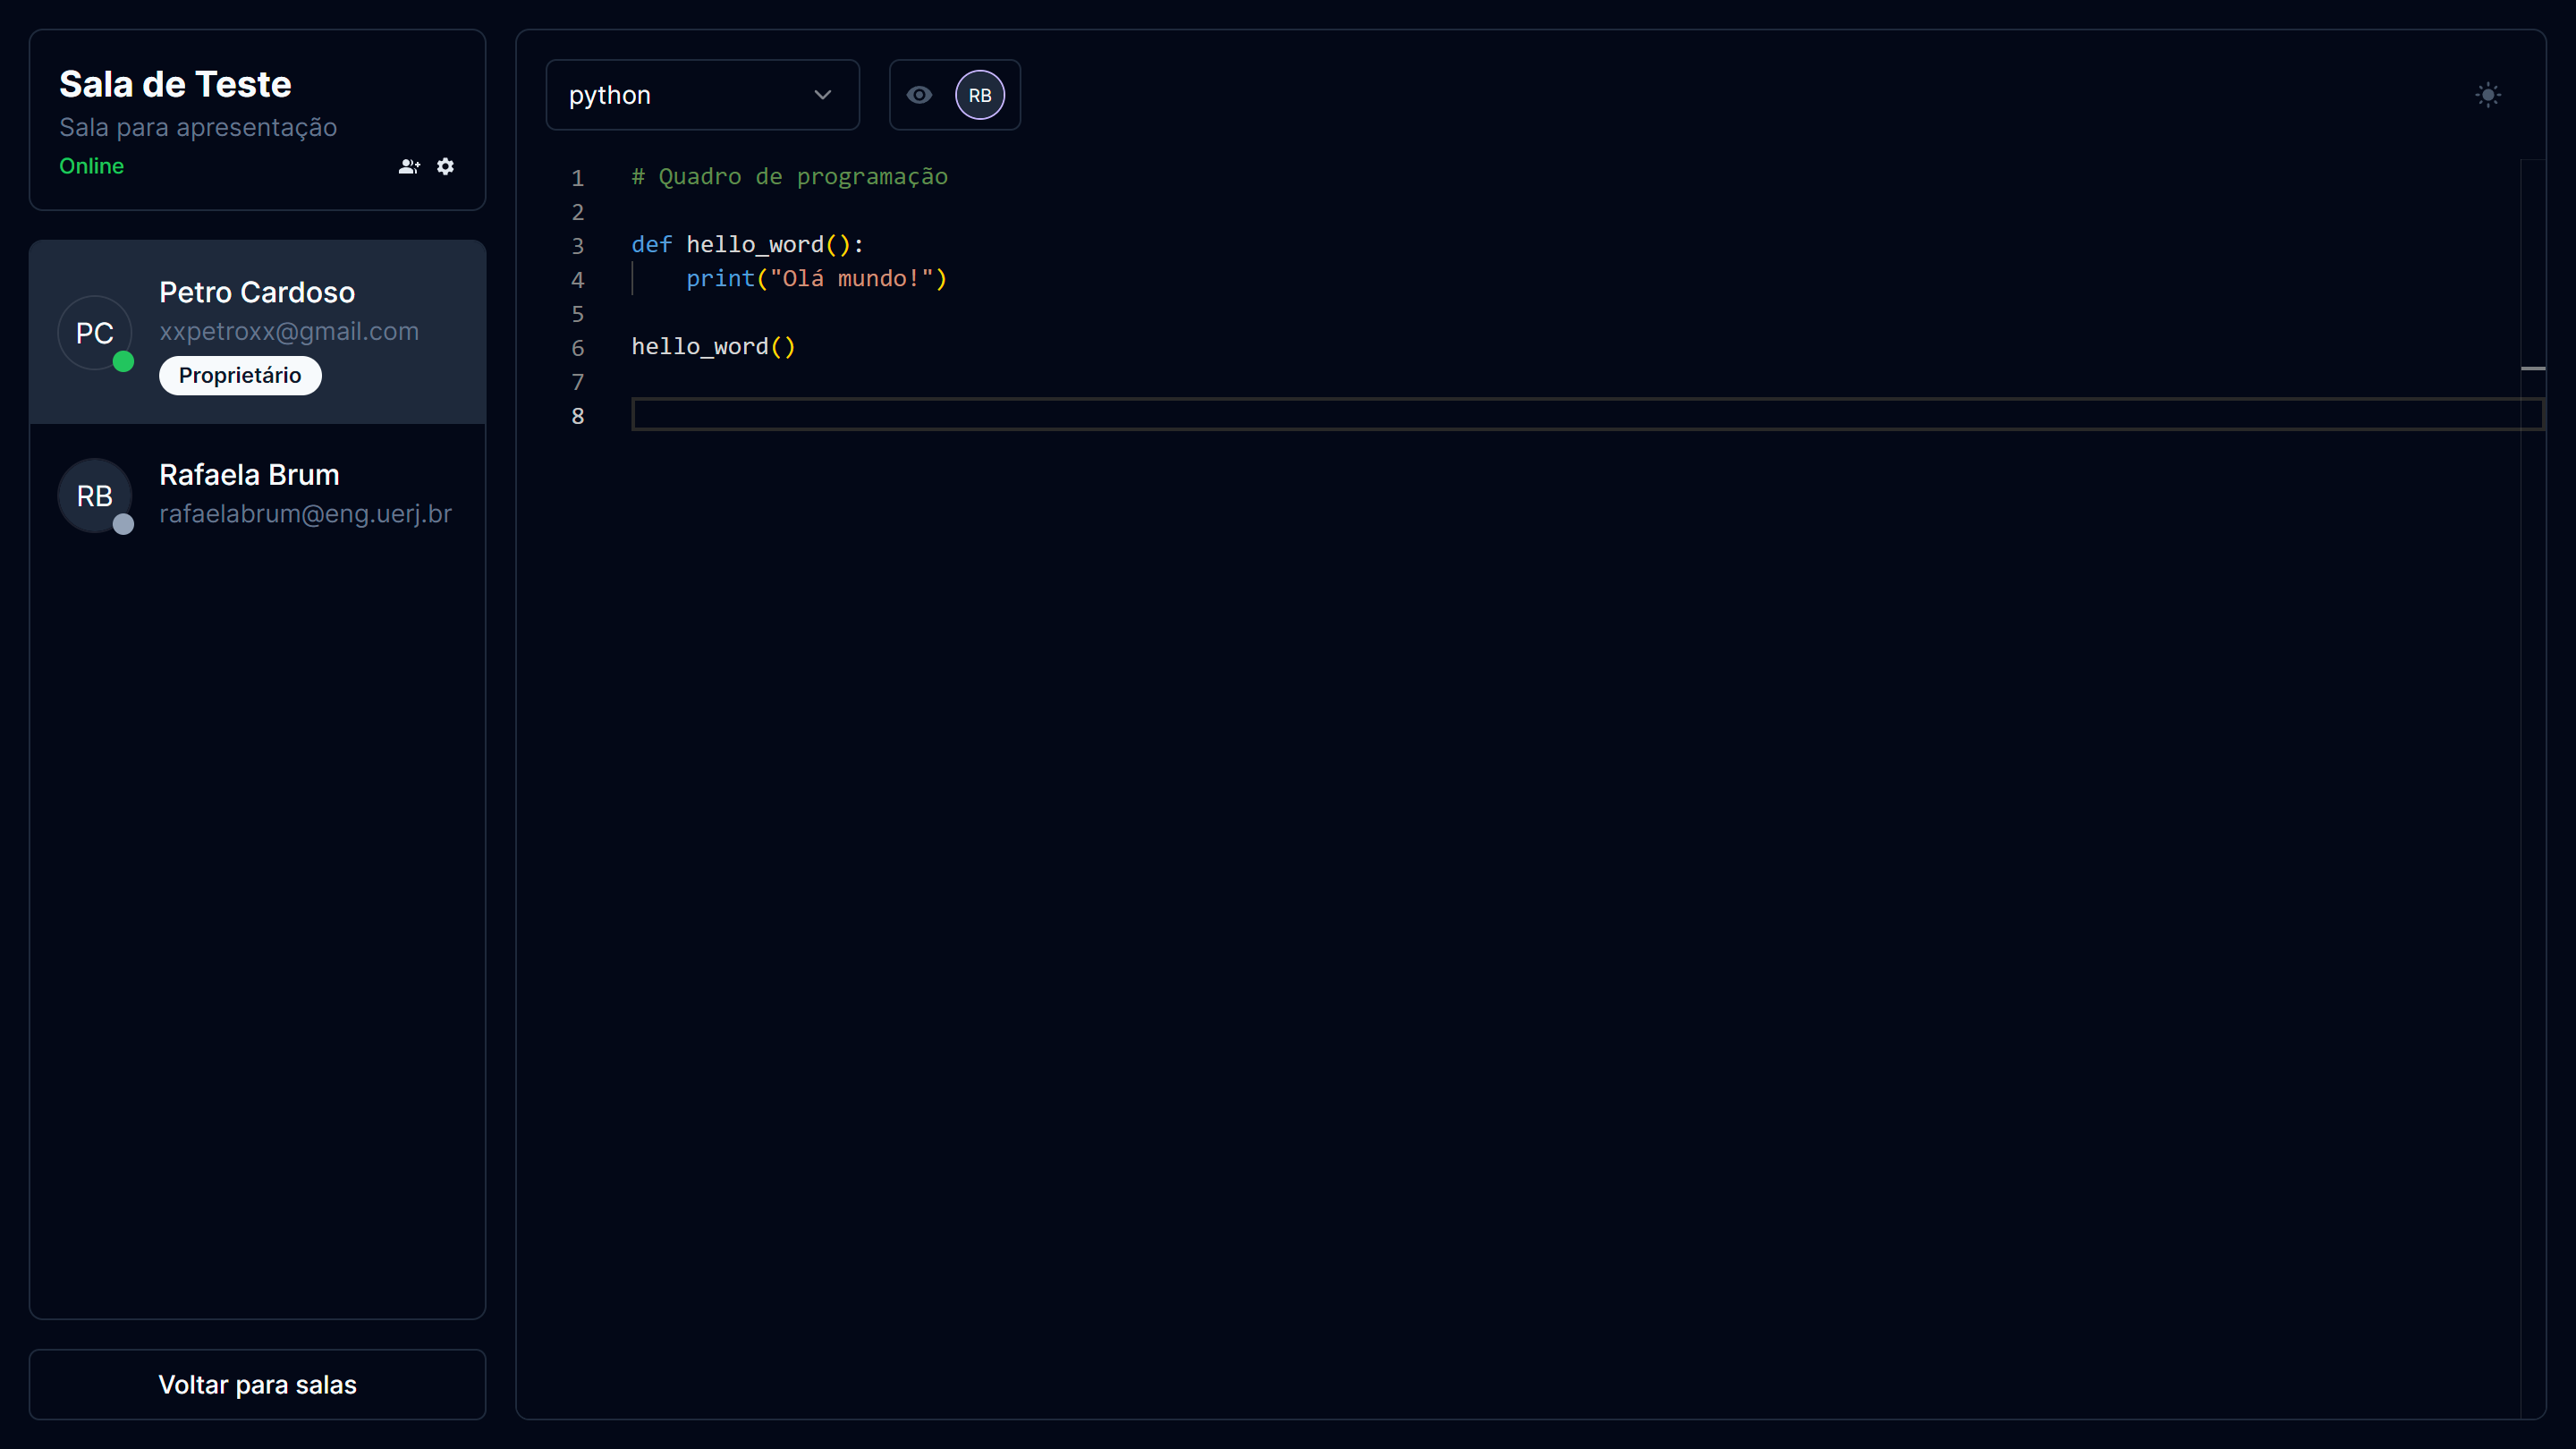
\includegraphics[width=1\textwidth]{assets/codeboard/room-details-page.png}
\end{figure}

Como mostrado na Figura \ref{fig:room-details-page}, o módulo lateral exibe a lista de participantes da sala, onde são apresentados o nome, a foto de perfil e indicadores que informam se o participante está online ou editando seu código. O usuário pode selecionar outro membro da sala para visualizar e interagir com o código dele em tempo real.

Caso o usuário selecione a si mesmo, ele poderá editar o próprio código, mudar a linguagem de programação e visualizar quem está acessando seu código. As edições são salvas automaticamente a cada modificação.

Acima do módulo lateral, o nome e a descrição da sala são exibidos. Se o usuário for o proprietário da sala, ele também verá os botões de adição de participantes e de configuração da sala. O botão de adição permite convidar novos membros, enquanto o botão de configuração possibilita a edição do nome e da descrição da sala. As figuras \ref{fig:add-member-modal} e \ref{fig:edit-room-modal} mostram os modais de adição de participantes e de configuração de sala, respectivamente.

\begin{figure}[H]{0.8\textwidth}
    \centering
    \caption{Modal de configuração de sala da plataforma Codeboard UERJ.}
    \label{fig:edit-room-modal}
    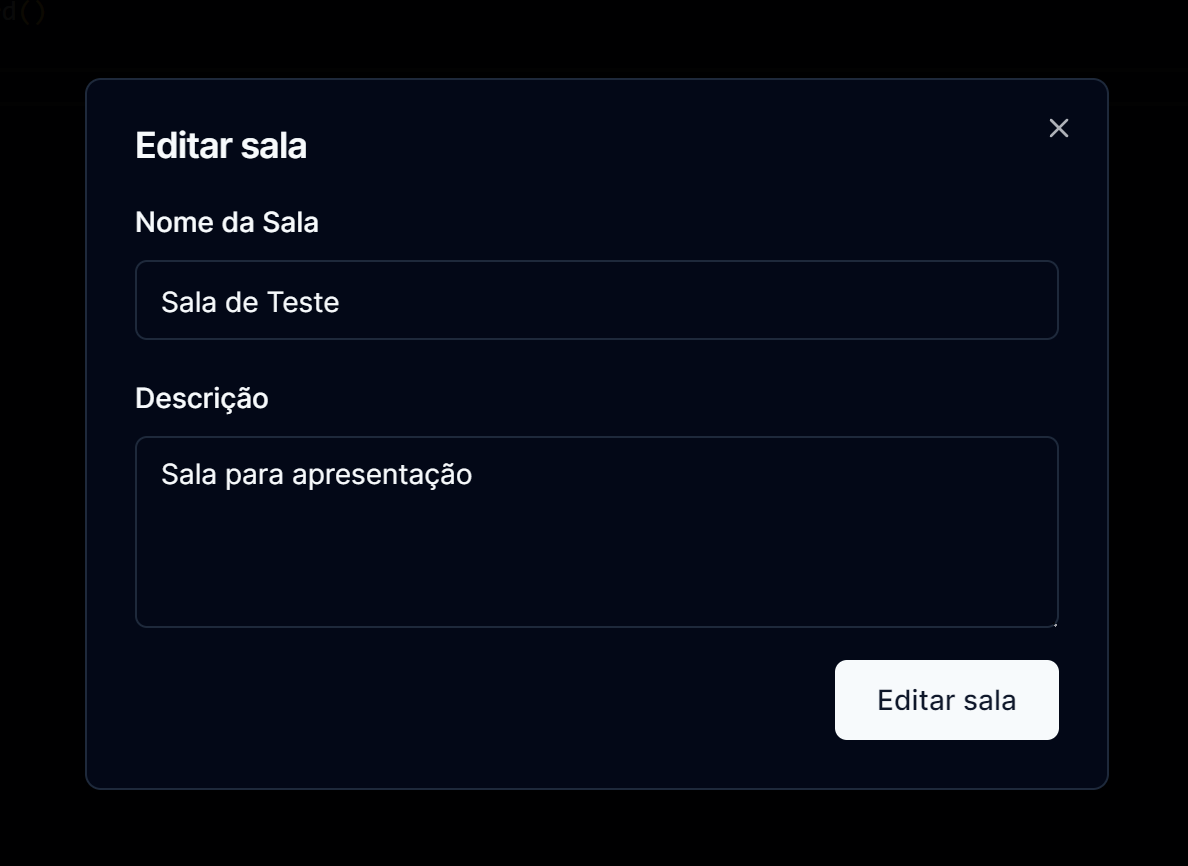
\includegraphics[width=0.8\textwidth]{assets/codeboard/edit-room-modal.png}
\end{figure}

Na parte inferior do módulo lateral, encontra-se o botão de saída, que redireciona o usuário de volta para a página de listagem de salas, onde ele pode acessar outras salas ou criar novas.

O módulo central abriga o editor de código, que oferece funcionalidades típicas de uma IDE, como coloração de sintaxe, auto-completar e formatação de código. Quando o usuário está visualizando o código de outro participante, ele pode fazer marcações visíveis em tempo real para todos os membros da sala, facilitando a comunicação e a colaboração. A Figura \ref{fig:code-editor-user-highlight} mostra um exemplo de marcação de código na plataforma.

\begin{figure}[H]{0.85\textwidth}
    \centering
    \caption{Marcação de código na plataforma Codeboard UERJ.}
    \label{fig:code-editor-user-highlight}
    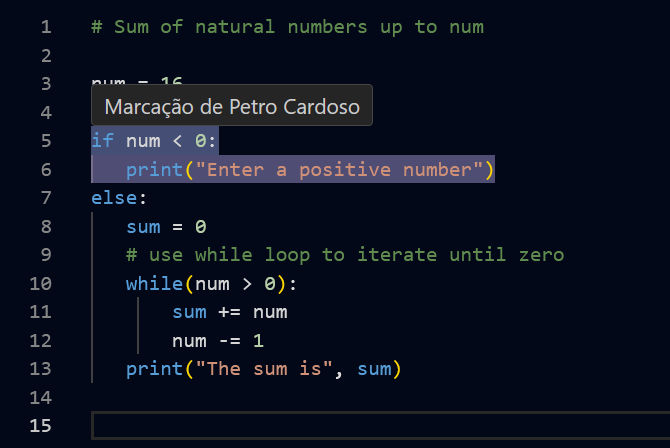
\includegraphics[width=0.85\textwidth]{assets/codeboard/code-editor-user-highlight.png}
\end{figure}

Na parte superior do editor, é possível selecionar a linguagem de programação desejada, com suporte para as linguagens mais utilizadas, como C, C++, Java, Python, Javascript etc. A escolha da linguagem altera a coloração de sintaxe, facilitando tanto a escrita quanto a leitura do código. 

Ao lado da seleção de linguagem, a plataforma exibe uma lista horizontal de quem está visualizando o código no momento, permitindo ao usuário monitorar em tempo real quem acompanha seu progresso.

A Figura \ref{fig:code-editor-toolbar} mostra a barra de ferramentas do editor de código, onde estão localizados os botões para seleção da linguagem de programação e para visualização dos usuários que estão acompanhando o quadro em tempo real.

\begin{figure}[H]{0.8\textwidth}
    \centering
    \caption{Barra de ferramentas do editor de código da plataforma.}
    \label{fig:code-editor-toolbar}
    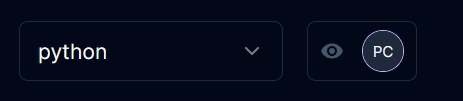
\includegraphics[width=0.8\textwidth]{assets/codeboard/code-editor-toolbar.png}
\end{figure}


\subsection{Regras de Negócio}

Existem algumas regras de negócio que devem ser seguidas para garantir o bom funcionamento da plataforma. Estas regras são implementadas no backend da plataforma e são responsáveis por validar os dados dos usuários e das salas, bem como garantir a segurança e a integridade dos dados.

\paragraph{Autenticação}

\begin{itemize}
    \item \textbf{Cadastro de Usuários}: A plataforma deve fornecer um mecanismo de registro que permita aos usuários criarem suas contas. Durante esse processo, serão solicitados dados como nome, e-mail e senha, que devem ser armazenados com segurança no banco de dados.
    \item \textbf{Validação de Dados}: É essencial que a plataforma assegure a qualidade e integridade das informações fornecidas pelos usuários. Isso inclui verificar a consistência dos dados durante o cadastro e o login, garantindo que apenas entradas válidas sejam aceitas.
    \item \textbf{Proteção de Dados}: Para resguardar as informações dos usuários, a plataforma deve aplicar técnicas de criptografia e hashing no armazenamento de dados sensíveis, prevenindo acessos não autorizados.
    \item \textbf{Login de Usuários}: O sistema de login deve verificar as credenciais informadas, como e-mail e senha, permitindo acesso apenas a usuários previamente cadastrados. Após a autenticação bem-sucedida, será gerado um token para manter a sessão ativa.
    \item \textbf{Gerenciamento de Sessões}: É fundamental administrar as sessões de forma eficiente, utilizando tokens de autenticação para identificar os usuários e encerrando sessões automaticamente após períodos prolongados de inatividade.
    \item \textbf{Restrição de Acesso}: Para proteger as funcionalidades da plataforma, o acesso deve ser limitado a usuários autenticados. A verificação da autenticação será realizada antes de liberar qualquer recurso ou serviço.
\end{itemize}

\paragraph{Gerenciamento de Salas}

\begin{itemize}
    \item \textbf{Criação de Salas}: A plataforma deve permitir que os usuários criem novas salas fornecendo informações como nome e descrição. Esses dados devem ser armazenados de forma segura no banco de dados.
    \item \textbf{Validação de Dados}: Para assegurar a integridade das informações, os dados das salas devem ser verificados durante os processos de criação e edição, garantindo consistência e validade.
    \item \textbf{Restrição de Acesso}: O acesso às salas será concedido apenas a participantes autorizados, com a confirmação de que o usuário é dono ou membro da sala antes de permitir a entrada.
    \item \textbf{Gerenciamento de Participantes}: Apenas usuários com permissões administrativas, como os proprietários das salas, poderão adicionar ou remover participantes.
    \item \textbf{Restrição de Edição}: A edição das informações da sala será limitada exclusivamente ao proprietário, mediante validação da propriedade antes de qualquer alteração.
\end{itemize}

\paragraph{Quadro de Programação}

\begin{itemize}
    \item \textbf{Editor em Tempo Real}: A plataforma deve disponibilizar um editor de código em tempo real, permitindo que os usuários programem diretamente no navegador. O editor deve incluir funcionalidades típicas de um IDE, como coloração de sintaxe, auto-completar e formatação de código.
    \item \textbf{Restrição de Escrita}: Conflitos durante a edição colaborativa serão evitados ao permitir que apenas o proprietário do código realize alterações, utilizando um mecanismo que bloqueia a escrita para os demais participantes
    \item \textbf{Marcação de Código}: O sistema deve possibilitar o destaque de trechos de código em tempo real, permitindo que os usuários acompanhem e interajam com as edições feitas por outros colaboradores no quadro.
    \item \textbf{Seleção de Linguagem}: A plataforma deve permitir a escolha da linguagem de programação diretamente no editor, ajustando automaticamente a coloração de sintaxe para a linguagem selecionada.
    \item \textbf{Visualização de Usuários}: Os usuários devem ter acesso a uma lista que mostre, em tempo real, quem está visualizando ou interagindo com o código no quadro.
\end{itemize}

\paragraph{Lista de Participantes}

\begin{itemize}
    \item \textbf{Visualização de Participantes}: A plataforma deve exibir uma lista que informe aos usuários quem está presente na sala, facilitando a identificação dos participantes ativos.
    \item \textbf{Indicadores de Presença}: Os usuários devem ter acesso a indicadores que mostrem quem está online e quem está editando o código no momento, tornando a colaboração mais clara e eficiente.
    \item \textbf{Seleção de Participantes}: Será possível selecionar participantes específicos para visualizar e interagir com o código deles, utilizando uma interface que permita essa escolha de forma simples e intuitiva.
\end{itemize}


\section{Implementação}
% Revisado

Nesta seção, será apresentada a implementação da plataforma Codeboard UERJ. A plataforma é estruturada em três componentes principais: o backend, o banco de dados e o frontend. Cada um deles desempenha um papel específico na plataforma, sendo responsável pelas regras de negócio, o armazenamento de dados e a interface com o usuário, respectivamente.

\subsection{Backend}
% Revisado

O backend da plataforma é responsável pela implementação das regras de negócio da aplicação. Ele é composto por um servidor NodeJS que utiliza dois métodos de comunicação: REST API e WebSockets. A REST API é usada para comunicação assíncrona entre o cliente e o servidor, enquanto os WebSockets são utilizados para permitir a comunicação em tempo real entre os usuários.

A comunicação entre o cliente e o servidor ocorre através de duas interfaces principais: REST API e WebSockets. A REST API fornece um conjunto de rotas que permitem ao cliente acessar funcionalidades da plataforma, como autenticação de usuários, gerenciamento de salas e edição de código. Os WebSockets, por sua vez, são utilizados para viabilizar a comunicação em tempo real entre os usuários, possibilitando a edição colaborativa de código. A Figura \ref{fig:backend-architecture} ilustra a arquitetura do backend da plataforma Codeboard UERJ.

\begin{figure}[H]{0.8\textwidth}
    \centering
    \caption{Arquitetura do backend da plataforma Codeboard UERJ.}
    \label{fig:backend-architecture}
    \includegraphics[width=0.75\textwidth]{diagrams/backend-architecture.png}
\end{figure}


\subsection{Banco de Dados NoSQL}
% Revisado

A plataforma utiliza o MongoDB, um banco de dados NoSQL orientado a documentos, devido à sua flexibilidade, escalabilidade horizontal e eficiência no armazenamento de grandes volumes de dados. Além disso, a integração simples com o NodeJS fez do MongoDB uma escolha natural para a plataforma Codeboard UERJ.

O banco de dados é estruturado em três coleções principais: a coleção de usuários (Users), a de salas (Rooms) e a de quadros de programação (Board). Essa organização está diretamente ligada às funcionalidades da plataforma, proporcionando armazenamento e recuperação eficazes dos dados dos usuários, das salas e dos quadros de programação. A Figura \ref{fig:database-schema} ilustra como essas coleções estão organizadas e como se relacionam no banco de dados.

\begin{figure}[H]{0.75\textwidth}
    \centering
    \caption{Esquema do banco de dados da plataforma.}
    \label{fig:database-schema}
    \includegraphics[width=0.75\textwidth]{diagrams/database-schema.png}
\end{figure}

A coleção de usuários armazena dados como nome, e-mail e senha dos usuários cadastrados. A Tabela \ref{tab:user-collection-fields} detalha os campos dessa coleção, que inclui:

\begin{itemize}
    \item \textbf{\_id}: Identificador único do usuário.
    \item \textbf{name}: Nome do usuário.
    \item \textbf{email}: E-mail do usuário.
    \item \textbf{password}: Hash da senha do usuário.
    \item \textbf{createdAt}: Data de criação do usuário.
\end{itemize}

\begin{table}[H]{1\textwidth}
    \centering
    \caption{Campos da coleção "User" do banco de dados da plataforma Codeboard UERJ.}
    \label{tab:user-collection-fields}
    \renewcommand{\arraystretch}{1.3} 
    \begin{tabular}{|c|c|c|c|}
        \hline
        \textbf{Campo}   & \textbf{Tipo} & \textbf{Obrigatório} \\
        \hline
        \_id            & ObjectId      & Sim                  \\
        \hline
        name              & String        & Sim                  \\
        \hline
        email              & String        & Sim                  \\
        \hline
        password         & String        & Sim                  \\
        \hline
        createdAt        & Date          & Sim                  \\
        \hline
    \end{tabular}
\end{table}

A coleção de usuários possui um campo password que armazena o hash da senha do usuário em vez da senha em texto puro. Essa prática garante a segurança dos dados, evitando que as senhas sejam armazenadas de forma insegura, o que poderia comprometer os usuários em caso de vazamento de informações.


A coleção de salas contém informações sobre as salas criadas, como nome, descrição e participantes. A Tabela \ref{tab:room-collection-fields} apresenta os campos dessa coleção, incluindo:

\begin{itemize}
    \item \textbf{\_id}: Identificador único da sala.
    \item \textbf{name}: Nome da sala.
    \item \textbf{description}: Descrição da sala.
    \item \textbf{owner}: Identificador do dono da sala.
    \item \textbf{members}: Lista de participantes da sala.
    \item \textbf{createdAt}: Data de criação da sala.
\end{itemize}

\begin{table}[H]{1\textwidth}
    \centering
    \caption{Campos da coleção "Room" do banco de dados da plataforma Codeboard UERJ.}
    \label{tab:room-collection-fields}
    \renewcommand{\arraystretch}{1.3} 
    \begin{tabular}{|c|c|c|c|}
        \hline
        \textbf{Campo}              & \textbf{Tipo}   & \textbf{Obrigatório} \\
        \hline
        \_id              & ObjectId        & Sim                  \\
        \hline
        name                          & String          & Sim                  \\
        \hline
        description               & String          & Não                  \\
        \hline
        owner          & ObjectId        & Sim                  \\
        \hline
        members        & Array<ObjectId> & Não                  \\
        \hline
        createdAt           & Date            & Sim                  \\
        \hline
    \end{tabular}
\end{table}


A coleção de quadros de programação armazena os códigos escritos pelos usuários, juntamente com a linguagem de programação utilizada. A Tabela \ref{tab:board-collection-fields} descreve os campos dessa coleção, que incluem:

\begin{itemize}
    \item \textbf{\_id}: Identificador único do quadro.
    \item \textbf{user}: Identificador do usuário dono do quadro.
    \item \textbf{room}: Identificador da sala do quadro.
    \item \textbf{language}: Linguagem de programação.
    \item \textbf{content}: Código de programação.
    \item \textbf{updatedAt}: Data da última atualização.
    \item \textbf{createdAt}: Data de criação.
\end{itemize}

\begin{table}[H]{1\textwidth}
    \centering
    \caption{Campos da coleção "Board" do banco de dados da plataforma Codeboard UERJ.}
    \label{tab:board-collection-fields}
    \renewcommand{\arraystretch}{1.3} 
    \begin{tabular}{|c|c|c|c|}
        \hline
        \textbf{Campo}             & \textbf{Tipo} & \textbf{Obrigatório} \\
        \hline
        \_id             & ObjectId      & Sim                  \\
        \hline
        user          & ObjectId      & Sim                  \\
        \hline
        room          & ObjectId      & Sim                  \\
        \hline
        language           & String        & Sim                  \\
        \hline
        content                 & String        & Sim                  \\
        \hline
        updatedAt         & Date          & Não                  \\
        \hline
        createdAt          & Date          & Sim                  \\
        \hline
    \end{tabular}
\end{table}

A coleção Board, possui os campos user e room, que contêm os identificadores do usuário proprietário do quadro e da sala à qual ele pertence, respectivamente. Esses relacionamentos garantem a organização dos dados e facilitam o gerenciamento de quadros de programação criados por diferentes usuários dentro de diferentes salas.

Apesar de o MongoDB ser um banco de dados NoSQL, a plataforma Codeboard UERJ segue um esquema de dados predefinido para garantir a consistência e integridade das informações armazenadas, ou seja, foram estabelecidos estruturas de dados pré-determinadas para cada coleção, especificando os campos, tipos de dados, relações entre diferentes coleções e regra de validação que cada documento deve seguir. Isso é fundamental para evitar inconsistências, como a inserção de dados inválidos ou incompletos, além de facilitar a manutenção e a evolução do sistema. Esse esquema é modelado e gerenciado no backend da plataforma com o auxílio da biblioteca \emph{Mongoose}, que simplifica o processo de modelagem e interação com o banco de dados MongoDB.


\subsection{Comunicação Síncrona via REST API}
% Revisado

A REST API é formada por um conjunto de rotas que possibilitam ao cliente acessar as funcionalidades da plataforma. Essas rotas são implementadas com o framework ExpressJS, que facilita a criação de rotas e middlewares em aplicações NodeJS.

Na REST API, existem três tipos principais de rotas: de autenticação, de usuários e de salas. As rotas de autenticação são responsáveis pela criação e autenticação de usuários, enquanto as rotas de usuários permitem o acesso e a atualização dos dados dos usuários. Já as rotas de salas são utilizadas para criar, acessar e gerenciar as salas.

A Tabela \ref{tab:rest-api-routes} apresenta as rotas da REST API da plataforma Codeboard UERJ, detalhando o método HTTP, a rota, sua descrição e se a autenticação é necessária para acessar cada uma delas.

\begin{table}[H]{1\textwidth}
    \centering
    \caption{Rotas da REST API da plataforma Codeboard UERJ.}
    \label{tab:rest-api-routes}
    \renewcommand{\arraystretch}{1.3} 
    \begin{tabular}{|c|c|c|c|}
        \hline
        \textbf{Método} & \textbf{Rota}                  & \textbf{Descrição}            & \textbf{Autenticação} \\
        \hline
        GET             & /api/health                    & Verifica o status do servidor & Não                   \\
        \hline
        POST            & /api/auth/signup               & Cadastra um novo usuário      & Não                   \\
        POST            & /api/auth/login                & Autentica um usuário          & Não                   \\
        \hline
        GET             & /api/user                      & Retorna os dados do usuário   & Sim                   \\
        PUT             & /api/user                      & Edita os dados do usuário     & Sim                   \\
        \hline
        GET             & /api/rooms                     & Lista todas as salas          & Sim                   \\
        POST            & /api/rooms                     & Cria uma nova sala            & Sim                   \\
        GET             & /api/rooms/:id                 & Retorna uma sala específica   & Sim                   \\
        PUT             & /api/rooms/:id                 & Edita uma sala específica     & Sim                   \\
        POST            & /api/rooms/:id/members         & Adiciona um membro à sala     & Sim                   \\
        DELETE          & /api/rooms/:id/members/:userId & Remove um membro da sala      & Sim                   \\
        \hline
    \end{tabular}
\end{table}


\subsection{Sistema de Autenticação}
% Revisado

As rotas descritas na Tabela \ref{tab:rest-api-routes} que requerem autenticação, são protegidas por um middleware que verifica se o usuário está autenticado antes de permitir o acesso. A autenticação do usuário na plataforma é realizada através de um token, que é gerado no servidor e enviado ao cliente após o login. 

O token de autenticação é gerado utilizando a biblioteca "jsonwebtoken", que implementa o padrão JWT (JSON Web Token). A escolha do JWT como mecanismo de autenticação foi motivada pela necessidade de suportar a infraestrutura horizontal da plataforma, que facilita a escalabilidade e a distribuição dos servidores. Como o JWT é um mecanismo \emph{stateless}, não é necessário armazenar o estado da sessão no servidor. Isso o torna ideal para aplicações distribuídas e escaláveis, pois o estado da sessão é armazenado no próprio token, que é enviado ao cliente.

O token é criado com base no ID do usuário e uma chave secreta, que é mantida nos servidores. Esse token é assinado com a chave secreta e enviado ao cliente, onde é armazenado no navegador por meio de cookies. A cada requisição feita ao servidor, o token é utilizado para autenticar o usuário, garantindo sua autenticidade em todas as páginas da plataforma.

O token de autenticação tem um tempo de expiração configurado no servidor. Após esse período, o token é invalidado, e o usuário é automaticamente desconectado da plataforma.


\subsection{Banco de Dados Chave-Valor}
% Revisado OK

A utilização do Redis na plataforma Codeboard UERJ foi necessária devido à sua natureza como uma ferramenta para colaboração em tempo real e comunicação descentralizada. A plataforma exige uma solução que permita a troca rápida e eficiente de informações, como a lista de usuários online, o código ativo nos quadros de programação e os visualizadores conectados, garantindo sincronização em tempo real entre os participantes.

O Redis foi escolhido principalmente por seu sistema de publicação/assinatura (pub/sub), que facilita a comunicação em tempo real, distribuindo atualizações de forma ágil e eficiente para múltiplos clientes. Além disso, suas características de alta eficiência, baixo tempo de resposta e suporte à escalabilidade horizontal tornam-no ideal para atender às demandas de velocidade e desempenho da Codeboard UERJ. A combinação dessas capacidades assegura que os dados temporários sejam gerenciados de maneira otimizada, reduzindo o consumo de recursos e aprimorando a experiência dos usuários.

O diagrama \ref{fig:redis-pubsub} a comunicação distribuída proporcionada pelo Redis utilizando o sistema de publicação/assinatura (Pub/Sub). Nele, dois servidores distintos (Servidor 1 e Servidor 2) interagem com o Redis, publicando mensagens em um canal específico. O Redis, por sua vez, distribui as mensagens recebidas para todos os servidores inscritos nesse canal, garantindo que as atualizações sejam propagadas em tempo real. Esse mecanismo é essencial para aplicações que necessitam de sincronização eficiente entre múltiplos pontos de processamento, como a plataforma Codeboard UERJ.

\begin{figure}[H]{1\textwidth}
    \centering
    \caption{Comunicação distribuída com Redis utilizando Pub/Sub.}
    \label{fig:redis-pubsub}
    \includegraphics[width=\textwidth]{diagrams/redis-pubsub.png}
\end{figure}


A adoção do Redis é comum em sistemas que demandam alta disponibilidade e tempos de resposta rápidos, características fundamentais para a experiência de colaboração simultânea proporcionada pela Codeboard UERJ. O Redis não apenas facilita a manipulação de dados em tempo real, mas também garante que os dados temporários sejam gerenciados de maneira eficiente, minimizando o uso excessivo de recursos.

A Tabela \ref{tab:key-value-database} descreve a estrutura do banco de dados chave-valor utilizado na plataforma, evidenciando como os dados são organizados em \emph{namespaces}. Cada \emph{namespace} reflete um contexto específico da aplicação, como as salas de colaboração ou os quadros de programação, e cada um possui um tempo de expiração associado, normalmente configurado para 1 dia. Essa expiração automática é essencial para a gestão de dados temporários e voláteis.

\begin{table}[H]{1\textwidth}
    \centering
    \caption{Estrutura do banco de dados chave-valor da plataforma.}
    \label{tab:key-value-database}
    \renewcommand{\arraystretch}{1.3} 
    \begin{tabular}{|c|p{6cm}|c|}
        \hline
        \textbf{Namespace}                   & \textbf{Descrição}                       & \textbf{Expiração} \\
        \hline
        room:\{roomId\}:users                & Lista de ID dos usuários online          & 1 dia              \\
        \hline
        board:\{roomId\}:\{boardId\}:code    & Código do quadro de programação          & 1 dia              \\
        \hline
        board:\{roomId\}:\{boardId\}:viewers & Lista de ID dos visualizadores do quadro & 1 dia              \\ 
        
        \hline
    \end{tabular}
\end{table}

O uso de \emph{namespaces} no Redis permite que diferentes componentes da plataforma sejam representados de forma hierárquica e clara. Por exemplo:
\begin{itemize}
    \item O \emph{namespace} \texttt{room:\{roomId\}:users} armazena os IDs dos usuários conectados a uma determinada sala, permitindo o rastreamento eficiente dos participantes ativos.
    \item O \emph{namespace} \texttt{board:\{roomId\}:\{boardId\}:code} contém o código do quadro de programação correspondente, garantindo que qualquer modificação seja rapidamente sincronizada entre os usuários.
    \item O \emph{namespace} \texttt{board:\{roomId\}:\{boardId\}:viewers} rastreia os visualizadores atuais de um quadro específico, permitindo o monitoramento em tempo real da audiência de cada quadro.
\end{itemize}

Todos esses dados são configurados para expirar após um dia de inatividade, removendo automaticamente informações temporárias que não são mais necessárias. A expiração controlada dos dados é crucial para manter o banco de dados eficiente e evitar acúmulo desnecessário de informações. Isso não só melhora o desempenho geral da plataforma, como também preserva a integridade do sistema ao evitar que informações desatualizadas sejam mantidas além do necessário.

Ao utilizar o Redis dessa maneira, a plataforma Codeboard UERJ assegura um ambiente escalável, rápido e confiável, adequado para as demandas de colaboração em tempo real.


\subsection{Comunicação em Tempo Real via WebSockets}

A plataforma Codeboard UERJ utiliza WebSockets para implementar comunicação em tempo real, permitindo a colaboração simultânea entre usuários na edição de código. Os WebSockets são uma tecnologia de comunicação bidirecional baseada em TCP, que possibilita a troca de mensagens entre clientes e servidores de maneira assíncrona e em tempo real. Essa abordagem elimina a necessidade de requisições HTTP constantes, facilitando o intercâmbio instantâneo de dados.

Para gerenciar as conexões WebSocket, a plataforma implementa \emph{middlewares} de autenticação, garantindo que apenas usuários autenticados possam se conectar e interagir. O processo de autenticação é realizado durante o estabelecimento da conexão, por meio de \emph{handshakes} que verificam a identidade do usuário através de tokens JWT. Dessa forma, apenas usuários devidamente autenticados e autorizados participam das interações em tempo real.

A comunicação em tempo real é estruturada em eventos e canais. Enquanto os eventos representam as mensagens trocadas entre os usuários, os canais funcionam como meios de comunicação, agrupando os usuários conforme o contexto da interação. Por exemplo, cada sala de programação possui seu próprio canal, onde os eventos são visíveis apenas para os usuários presentes, garantindo a privacidade e segurança das interações.

Além disso, os canais podem conter subcanais, permitindo a criação de hierarquias de comunicação. Por exemplo, uma sala de programação pode incluir subcanais dedicados a quadros específicos, facilitando uma comunicação segmentada e específica entre os usuários de cada quadro.

A Tabela \ref{tab:websocket-client-to-server-events}  lista os principais eventos que os clientes da plataforma Codeboard UERJ enviam ao servidor por meio de WebSockets, junto com suas respectivas descrições. Esses eventos possibilitam a interação dos usuários com as salas de programação, os quadros de edição de código e outros participantes, viabilizando a colaboração em tempo real.

\begin{table}[H]{1\textwidth}
    \centering
    \caption{Eventos WebSocket enviados do cliente para o servidor na plataforma.}
    \label{tab:websocket-client-to-server-events}
    \renewcommand{\arraystretch}{1.3} 
    \begin{tabular}{|c|p{10cm}|}
        \hline
        \textbf{Evento} & \textbf{Descrição} \\
        \hline
        \texttt{room:join} & Emitido pelo usuário quando ele entra em uma sala. É enviado no corpo da mensagem o ID da sala. \\
        \hline
        \texttt{board:join} & Emitido pelo usuário quando ele entra em um quadro de programação. É enviado no corpo da mensagem o ID da sala e do quadro de programação. \\
        \hline
        \texttt{board:leave} & Emitido pelo usuário quando ele sai de um quadro de programação. É enviado no corpo da mensagem o ID da sala e do quadro de programação. \\
        \hline
        \texttt{board:write} & Usado quando um usuário começa a digitar ou modificar o código no quadro. É enviado no corpo da mensagem o conteúdo do código e o ID do quadro de programação. \\
        \hline
        \texttt{board:highlight} & Usado para destacar partes específicas do código. É enviado no corpo da mensagem a posição do cursor, o ID da sala e do quadro de programação. \\
        \hline
        \texttt{board:read} & Usado para solicitar o conteúdo de um quadro de programação para visualização. É enviado no corpo da mensagem o ID da sala e do quadro de programação. \\
        \hline
    \end{tabular}
\end{table}


A Tabela \ref{tab:websocket-server-to-client-events} apresenta os eventos enviados pelo servidor da plataforma Codeboard UERJ aos clientes, juntamente com suas descrições. Esses eventos permitem que os usuários acompanhem, em tempo real, as atividades e interações dos outros participantes, assegurando a sincronia durante a colaboração.

\begin{table}[H]{1\textwidth}
    \centering
    \caption{Eventos WebSocket enviados do servidor para o cliente na plataforma.}
    \label{tab:websocket-server-to-client-events}
    \renewcommand{\arraystretch}{1.3} 
    \begin{tabular}{|c|p{10cm}|}
        \hline
        \textbf{Evento} & \textbf{Descrição} \\
        \hline
        \texttt{room:joined} & Emitido pelo servidor quando um novo usuário ficou online na sala, informando quem é o novo membro. \\
        \hline
        \texttt{room:members} & Emitido logo após o usuário entrar na sala, informando quem são os outros membros da sala. \\
        \hline
        \texttt{board:joined} & Informa que um usuário entrou no quadro de programação selecionado. \\
        \hline
        \texttt{board:viewers} & Emitido após um usuário entrar no quadro de programação, informando quem são os outros visualizadores. \\
        \hline
        \texttt{board:left} & Indica que um usuário saiu do quadro de programação selecionado. \\
        \hline
        \texttt{board:typed} & Indica que um usuário está digitando no quadro de programação. \\
        \hline
        \texttt{board:written} & Emite o conteúdo do código escrito do quadro de programação. \\
        \hline
        \texttt{board:highlighted} & Informa a todos os usuários a localização exata da marcação feita por um usuário no quadro de programação selecionado. \\
        \hline
    \end{tabular}
\end{table}

A Tabela \ref{tab:websocket-server-control-events} apresenta os eventos de controle de conexão na plataforma Codeboard UERJ, acompanhados de suas descrições. Esses eventos são responsáveis por gerenciar o estabelecimento e a finalização das conexões WebSocket entre os clientes e o servidor.

\begin{table}[H]{1\textwidth}
    \centering
    \caption{Eventos WebSocket enviados do cliente para o servidor na plataforma.}
    \label{tab:websocket-server-control-events}
    \renewcommand{\arraystretch}{1.3} 
    \begin{tabular}{|c|p{10cm}|}
        \hline
        \textbf{Evento} & \textbf{Descrição} \\
        \hline
        \texttt{connect} & Evento base disparado quando um novo cliente estabelece uma conexão com o WebSocket. \\
        \hline
        \texttt{disconnecting} & Acionado quando um usuário está prestes a perder a conexão. \\
        \hline
    \end{tabular}
\end{table}


Para visualizar o fluxo dessas interações, o diagrama de sequência da Figura \ref{fig:websocket-flow} exemplifica a comunicação em tempo real da comunicação entre o \textbf{usuário}, o \textbf{servidor} e outros usuários que participam de uma \textbf{sala} ou de um \textbf{quadro de programação} na plataforma, destacando pontos críticos de interação e troca de informações.

\begin{figure}[H]{1\textwidth}
    \centering
    \caption{Diagrama de sequência da comunicação em tempo real na plataforma.}
    \label{fig:websocket-flow}
    \makebox[\textwidth]{\includegraphics[width=0.9\paperwidth]{diagrams/websocket-flow.png}}
\end{figure}

 O fluxo de comunicação é dividido em etapas distintas, cada uma representando uma ação específica realizada pelo usuário ou pelo servidor:

\begin{enumerate}
    \item \textbf{Autenticação do Usuário}:
    \begin{itemize}
        \item O \textbf{usuário} inicia a conexão enviando o evento \texttt{connect} para estabelecer a comunicação WebSocket com o servidor. Após validar a autenticação, o \textbf{servidor} responde com o evento \texttt{connected}, confirmando a conexão.
        \item Caso a autenticação falhe, o \textbf{servidor} emite o evento \texttt{error}, sinalizando que o acesso foi negado.
    \end{itemize}

    \item \textbf{Entrada na Sala}:
    \begin{itemize}
        \item O \textbf{usuário} entra em uma sala de programação enviando o evento \texttt{room:join} ao \textbf{servidor}, que, por sua vez, notifica os demais \textbf{usuários da sala} sobre sua chegada com o evento \texttt{room:joined}.
        \item O \textbf{servidor} também envia ao \textbf{usuário} a lista atual de participantes da sala por meio do evento \texttt{room:members}.
    \end{itemize}

    \item \textbf{Entrada no Quadro de Programação}:
    \begin{itemize}
        \item Ao acessar um quadro de programação, o \textbf{usuário} envia o evento \texttt{board:join}. O \textbf{servidor} notifica os demais \textbf{usuários do quadro} com o evento \texttt{board:joined} e simultaneamente envia ao \textbf{usuário} entrante uma lista dos visualizadores atuais por meio do evento \texttt{board:viewers}.
    \end{itemize}

    \item \textbf{Edição de Código}:
    \begin{itemize}
        \item Quando o \textbf{usuário} começa a modificar o código no quadro, o evento \texttt{board:write} é enviado ao \textbf{servidor}. O \textbf{servidor} então informa para os demais \textbf{usuários da sala} que aquele usuário está digitando (\texttt{board:typed}), simultaneamente ele também transmite o conteúdo atualizado do código para todos os \textbf{usuários do quadro} com o evento \texttt{board:written}.
    \end{itemize}

    \item \textbf{Destaque de Código}:
    \begin{itemize}
        \item O \textbf{usuário} pode destacar partes do código enviando o evento \texttt{board:highlight} para o \textbf{servidor}. Este, por sua vez, notifica a todos os \textbf{usuários do quadro} sobre a posição exata do destaque com o evento \texttt{board:highlighted}.
    \end{itemize}

    \item \textbf{Desconexão}:
    \begin{itemize}
        \item Quando o \textbf{usuário} decide sair da plataforma, o evento \texttt{disconnecting} é enviado ao \textbf{servidor}, que informa tanto para os \textbf{usuários do quadro} (com o evento \texttt{board:left}) quanto para os \textbf{usuários da sala} (com o evento \texttt{room:left}) sobre a saída do participante.
    \end{itemize}
\end{enumerate}

Esse diagrama reflete a sequência de eventos que possibilitam a colaboração em tempo real entre usuários da plataforma, garantindo a sincronia e atualização constante dos dados compartilhados durante o uso.


\subsection{Comunicação Assíncrona via Filas}
% REVISADO

A plataforma Codeboard UERJ utiliza um sistema de filas para processar tarefas assíncronas, como o salvamento de código após a desconexão de um usuário. Esse sistema é composto por um servidor principal e \emph{workers}, que são responsáveis por executar as tarefas em segundo plano.

O servidor principal é responsável por receber as requisições dos clientes, autenticar os usuários, gerenciar as conexões WebSocket e distribuir as tarefas para os workers. Os workers, por sua vez, são responsáveis por processar as tarefas assíncronas, como salvar o código de um quadro de programação após a desconexão de um usuário.

A comunicação entre o servidor principal e os workers é feita através de filas, que são gerenciadas pelo sistema de envio e recebimento de mensagens da Amazon, o AWS SQS. 

Quando uma tarefa assíncrona precisa ser executada, o servidor principal a enfileira na fila correspondente uma mensagem, indicando o tipo de tarefa e os parâmetros necessários para sua execução. Os workers, por sua vez, ficam monitorando as filas por meio de \emph{long polling}, verificando se existem mensagens a serem processadas. Quando uma mensagem é encontrada, o worker a recebe, executa a operação correspondente e posteriormente a remove da fila.

Caso ocorra algum erro durante a execução da tarefa, o worker pode aguardar um tempo determinado e tentar executar a tarefa novamente. Caso ainda assim não seja possível concluir a tarefa, o worker irá remover a tarefa da fila e a enviará para uma DLQ (Dead Letter Queue), onde as tarefas que não puderam ser processadas são armazenadas para posterior análise e tratamento.

O fluxo de comunicação assíncrona via filas é ilustrado no diagrama de sequência da Figura \ref{fig:queue-flow}, que exemplifica a interação entre o \textbf{servidor principal}, os \textbf{workers} e as \textbf{filas}.

\begin{figure}[H]{1\textwidth}
    \centering
    \caption{Diagrama de sequência da comunicação assíncrona via filas na plataforma.}
    \label{fig:queue-flow}
    \makebox[\textwidth]{\includegraphics[width=0.95\paperwidth]{diagrams/queue-flow.png}}
\end{figure}

Essa abordagem de comunicação assíncrona via filas é essencial para que a plataforma Codeboard UERJ processe tarefas de salvamento de código com eficiência, escalabilidade e resiliência. A eficiência assegura que as operações sejam concluídas sem atrasos, mesmo em um ambiente de alta interação e colaboração em tempo real. A escalabilidade permite que o sistema gerencie aumentos de carga, como em horários de pico, adaptando-se ao número de usuários e à complexidade das tarefas. Por fim, a resiliência garante a integridade das operações ao lidar com falhas, utilizando mecanismos como reprocessamento e Dead Letter Queues, preservando a confiabilidade da plataforma e a segurança dos dados dos usuários.


\subsection{Interface do Usuário}

O frontend da plataforma Codeboard UERJ foi desenvolvido com o objetivo de oferecer uma interface intuitiva, eficiente e escalável. Para alcançar esse objetivo, foi utilizada uma \emph{stack} de tecnologias modernas, composta principalmente por ReactJS, Next.js, Tailwind CSS e shadcn/ui. A escolha dessas ferramentas visou a criação de um ambiente de desenvolvimento ágil e um resultado final otimizado para a experiência do usuário.

Next.js foi escolhido como o \emph{framework} principal para a construção do frontend, devido às suas capacidades de Static Site Generation (SSG). Essa característica permite que a plataforma carregue páginas de forma rápida e eficiente, ao mesmo tempo em que melhoravam o SEO e a experiência de navegação dos usuários. Além disso, o Next.js oferece suporte nativo a React, facilitando a criação de componentes reutilizáveis e a organização do código.

A estilização da plataforma foi realizada com Tailwind CSS, um framework de utilitários CSS que facilita a criação de interfaces responsivas e customizáveis. A escolha do Tailwind possibilitou uma organização clara dos estilos, sem a necessidade de escrever CSS adicional, aumentando a eficiência do processo de desenvolvimento. Além disso, o uso de classes utilitárias do Tailwind permitiu a rápida criação de componentes reativos e responsivos, otimizando o layout para diferentes tamanhos de tela.

Para a construção de componentes reutilizáveis, a plataforma integrou o shadcn/ui, um conjunto de componentes customizados que foram utilizados em elementos interativos como botões, modais e formulários. Essa abordagem facilitou a manutenção do código e garantiu uma coesão visual em toda a interface.

% TODO: Rever acessibilidade na plataforma com o uso de softwares de leitura de tela e outras ferramentas de acessibilidade.
Outro aspecto fundamental foi a acessibilidade. A plataforma foi desenvolvida com foco em garantir que todos os usuários, independentemente de suas limitações, pudessem interagir com a plataforma. Foram seguidas boas práticas de design acessível, incluindo o uso de atributos ARIA e a criação de componentes navegáveis via teclado, que facilitam a interação com softwares de leitura de tela e outras ferramentas de acessibilidade.

Essa abordagem de desenvolvimento garantiu que a plataforma Codeboard UERJ oferecesse uma experiência de uso fluida, responsiva e acessível, além de facilitar a manutenção e escalabilidade do projeto no longo prazo.

